% --------------------------------------------------------------
% This is all preamble stuff that you don't have to worry about.
% Head down to where it says "Start here"
% --------------------------------------------------------------
 
\documentclass[12pt]{article}
 
\usepackage[margin=1in]{geometry} 
\usepackage{amsmath,amsthm,amssymb,mathtools}
\usepackage{enumerate} 
\usepackage{graphicx,float} % figures
\usepackage{csvsimple,longtable,booktabs} % load csv as a table
\usepackage{listings,color} % for code snippets


\newenvironment{proposition}[2][Proposition]{\begin{trivlist}
\item[\hskip \labelsep {\bfseries #1}\hskip \labelsep {\bfseries #2.}]}{\end{trivlist}}

 
%%======%%
% All this is to force LaTeX to prefix "Appendix" before a new appendix section letter
\makeatletter
% The "\@seccntformat" command is an auxiliary command
% (see pp. 26f. of 'The LaTeX Companion,' 2nd. ed.)
\def\@seccntformat#1{\@ifundefined{#1@cntformat}%
   {\csname the#1\endcsname\quad}  % default
   {\csname #1@cntformat\endcsname}% enable individual control
}
\let\oldappendix\appendix %% save current definition of \appendix
\renewcommand\appendix{%
    \oldappendix
    \newcommand{\section@cntformat}{\appendixname~\thesection\quad}
}
\makeatother
%%======%%

%%======%%
% Define for code section
\definecolor{dkgreen}{rgb}{0,0.6,0}
\definecolor{gray}{rgb}{0.5,0.5,0.5}
\definecolor{mauve}{rgb}{0.58,0,0.82}

\lstset{frame=tb,
  language=C++,
  aboveskip=3mm,
  belowskip=3mm,
  showstringspaces=false,
  columns=flexible,
  basicstyle={\footnotesize\ttfamily},
  numbers=none,
  numberstyle=\tiny\color{gray},
  keywordstyle=\color{blue},
  commentstyle=\color{dkgreen},
  stringstyle=\color{mauve},
  breaklines=true,
  breakatwhitespace=true,
  tabsize=3
}
%%======%%


\begin{document}
 
% --------------------------------------------------------------
%                         Start here
% --------------------------------------------------------------
 
\title{Assignment 1}
\author{David Fleischer\\ 
MACF 402 - Mathematical \& Computational Finance II}
 
\maketitle
\noindent {\bf Question 1}. Show that \\
\begin{align}
u = e^{R\Delta t}(1 + \sqrt{e^{\sigma^2\Delta t} - 1}) \label{q1u} \\
d = e^{R\Delta t}(1 - \sqrt{e^{\sigma^2\Delta t} - 1}) \label{q1d}
\end{align}
is equivalent to
\begin{align*}
u = 1 + \sigma\sqrt{\Delta t} + R\Delta t + \mathcal O(\Delta t^{^3/_2}) \\
d = 1 + \sigma\sqrt{\Delta t} - R\Delta t + \mathcal O(\Delta t^{^3/_2})
\end{align*}
for constant $R, \sigma$, as $\Delta t \longrightarrow 0$ \\

\noindent {\bf Solution}. For brevity, let
\begin{equation*}
^u_d =  \sigma\sqrt{\Delta t} \pm R\Delta t + \mathcal O(\Delta t^{^3/_2})
\end{equation*}
\noindent denote the system
\begin{align*}
    \left\{
                \begin{array}{ll}
u = 1 + \sigma\sqrt{\Delta t} + R\Delta t + \mathcal O(\Delta t^{^3/_2}) \\
d = 1 + \sigma\sqrt{\Delta t} - R\Delta t + \mathcal O(\Delta t^{^3/_2})
                \end{array}
              \right.
\end{align*}
\\
\\
\noindent First, by Taylor's Theorem, if $f$ has a continuous derivative up to order 2 then,
\begin{equation*}
	f(x) = f(0) + xf'(0) + \frac{1}{2}x^2f''(\xi) 	
\end{equation*}
where $\xi \in [0,x]$. Assume $x \in [-1,1]$ so that $f''(\xi)$ is bound by some constant then,
\begin{equation*}
	f(x) = f(0) + xf'(0) + \mathcal O(x^2)
\end{equation*}
So, for $|x|$ sufficiently small,
\begin{align}
	e^x & = 1 + x + \mathcal O(x^2) \label{exp} \\
	\sqrt{1 + x} & = 1 + \frac{1}{2}x + \mathcal O(x^2) \label{sqrt}
\end{align}

\noindent Next, we introduce some useful properties of $\mathcal O(\cdot)$. Recall that, as $x \longrightarrow 0^+$, we say $f(x)$ is of the order $g(x)$ (denoted $f(x) = \mathcal O(g(x)))$ if $\exists c,x_0 \in \mathbb{R}^{+}: 0 \leq f(x) \leq cg(x)$ for all $x \leq x_0$. So, consider $x \longrightarrow 0^+$ and $c_1, c_2, k \in \mathbb{R^+}$,
\begin{enumerate}
\item If $f(x) = c_1\mathcal O(g(x))$ then, %%%% property 1
\begin{align*}
	c_1\mathcal O(g(x)) = c_1c_2g(x) = kg(x) 
\end{align*}
So we have $f(x) = c_1\mathcal O(g(x))$ bound by $kg(x)$. That is,
\begin{equation*}
	f(x) = c_1\mathcal O(g(x)) = \mathcal O(g(x))
\end{equation*}

\item If $f(x) = g_1(x)\mathcal O(g_2(x))$ then, %%% property 2
 \begin{align*} 
	g_1(x)\mathcal O(g_2(x)) & \leq g_1(x)kg_2(x) = kg_1(x)g_2(x)
\end{align*} 
So we have $g_1(x)\mathcal O(g_2(x))$ bound by $kg_1(x)g_2(x)$, so it is of the order $g_1(x)g_2(x)$. That is, 
\begin{equation*}
	f(x) = g_1(x)\mathcal O(g_2(x)) = \mathcal O(g_1(x)g_2(x))
\end{equation*}

\item If $f(x) = \mathcal O(\mathcal O(x)^{^n/_m})$ then, %%% property 3
\begin{align*}
	\mathcal O (\mathcal O(x)^{^n/_m}) & \leq c_1\mathcal O(x)^{^n/_m} \\
	& \leq c_1(c_2x)^{^n/_m} = c_1c_2^{^n/_m}x^{^n/_m} = kx^{^n/_m}
\end{align*}
So we have $\mathcal O(\mathcal O(x)^{^n/_m})$ bound by $kx^{^n/_m}$, so it is of the order $x^{^n/_m}$. That is,
\begin{equation*}
	f(x) = \mathcal O(\mathcal O(x)^{^n/_m}) = \mathcal O(x^{^n/_m})
\end{equation*}

\item If $f_1(x) = \mathcal O(g_1(x))$ and $f_2(x) = \mathcal O(g_2(x))$ then,  %%% property 4
\begin{align*}
	\mathcal O(g_1(x)) + \mathcal O(g_2(x)) &\leq c_1g_1(x) + c_2g_2(x) \\
	&\leq max(c_1,c_2)(g_1(x) + g_2(x)) = k(g_1(x) + g_2(x))
\end{align*}
So we have $\mathcal O(g_1(x)) + \mathcal O(g_2(x)) $ bound by $k(g_1(x) + g_2(x))$, so it is of the order $g_1(x) + g_2(x)$. That is, \\
\begin{equation*}
	f(x) = \mathcal O(g_1(x)) + \mathcal O(g_2(x)) = \mathcal O(g_1(x) + g_2(x))
\end{equation*} \\
\end{enumerate} 
\noindent Now that we've set up our playing field we may evaluate the terms $e^{R\Delta t}$ and $e^{\sigma^2\Delta t}$ in (\ref{q1u}) \& (\ref{q1d}) at $x = R\Delta t$ and $x = \sigma^2\Delta t$, respectively. This leaves us with,
\begin{align*}
	^u_d & = (1 + R\Delta t + \mathcal O(R^2\Delta t^2))(1 \pm \sqrt{1 + \sigma^2\Delta t + \mathcal O(\sigma^4\Delta t^2) - 1}) \\
	& =  (1 + R\Delta t + \mathcal O(R^2\Delta t^2))(1 \pm \sqrt{\sigma^2\Delta t + \mathcal O(\sigma^4\Delta t^2)})
\end{align*}

\noindent Using the properties of $\mathcal O(\cdot)$ introduced above, for $\Delta t \longrightarrow 0^+$,
\begin{align*}
	^u_d  & =  (1 + R\Delta t + \mathcal O(R^2\Delta t^2))(1 \pm \sqrt{\sigma^2\Delta t + \mathcal O(\sigma^4\Delta t^2)}) \\
	& = (1 + R\Delta t + \mathcal O(\Delta t^2))(1 \pm \sqrt{\sigma^2\Delta t + \mathcal O(\Delta t^2)}) \quad (\text{by Property 1}) \\
	& = (1 + R\Delta t + \mathcal O(\Delta t^2))(1 \pm \sqrt{\sigma^2\Delta t + \Delta t \mathcal O(\Delta t)}) \quad (\text{by Property 2}) \\
	& = (1 + R\Delta t + \mathcal O(\Delta t^2))(1 \pm \sigma\sqrt{\Delta t}\sqrt{1 + \frac{1}{\sigma^2}\mathcal O(\Delta t)}) \\
	& = (1 + R\Delta t + \mathcal O(\Delta t^2))(1 \pm \sigma\sqrt{\Delta t}\sqrt{1 + \mathcal O(\Delta t)}) \quad (\text{by Property 1}) \\
\end{align*}
Evaluating (\ref{sqrt}) at $x = \mathcal O(\Delta t)$ we have,
\begin{align*}
	^u_d  & = (1 + R\Delta t + \mathcal O(\Delta t^2))(1 \pm \sigma\sqrt{\Delta t}(1 + \frac{1}{2}\mathcal O(\Delta t) + \mathcal O(\mathcal O(\Delta t)^2)) \\
	& = (1 + R\Delta t + \mathcal O(\Delta t^2))(1 \pm \sigma\sqrt{\Delta t}(1 + \mathcal O(\Delta t) + \mathcal O(\mathcal O(\Delta t)^2)) \quad (\text{by Property 1}) \\
	& = (1 + R\Delta t + \mathcal O(\Delta t^2))(1 \pm \sigma\sqrt{\Delta t}(1 + \mathcal O(\Delta t) + \mathcal O(\Delta t^2)) \quad (\text{by Property 3}) \\
	& = (1 + R\Delta t + \mathcal O(\Delta t^2))(1 \pm \sigma\sqrt{\Delta t}(1 + \mathcal O(\Delta t + \Delta t^2)) \quad (\text{by Property 4}) \\
\end{align*}

\noindent We see that $\mathcal O(\Delta t + \Delta t^2)$ = $\mathcal O(\Delta t)$ (as $\Delta t \longrightarrow 0^+$) since we may find some positive constant $k$ such that $\Delta t + \Delta t^2 \leq k\Delta t$. So,
\begin{align*}
	^u_d & = (1 + R\Delta t + \mathcal O(\Delta t^2))(1 \pm \sigma\sqrt{\Delta t}(1 + \mathcal O(\Delta t)) \\
	& = (1 + R\Delta t + \mathcal O(\Delta t^2))(1 \pm \sigma\sqrt{\Delta t} \pm \sigma\sqrt{\Delta t}\mathcal O(\Delta t)) \\ 
	& = (1 + R\Delta t + \mathcal O(\Delta t^2)(1 \pm \sigma\sqrt{\Delta t} + \mathcal O(\Delta t^{^3/_2})) \quad \text{(by Properties 1 \& 2)} \\
	& = 1 + R\Delta t + \mathcal O(\Delta t^2) \pm \sigma\sqrt{\Delta t} \pm R\Delta t\sigma\sqrt{\Delta t} \pm \mathcal O(\Delta t^2)\sigma\sqrt{\Delta t} \\ & \phantom{\hfill{12cm}} + \mathcal O(\Delta t^{^3/_2}) + R\Delta t\mathcal O(\Delta t^{^3/_2}) + \mathcal O(\Delta t^2)\mathcal O(\Delta t^{^3/_2}) \\
	& = 1 + R\Delta t + \mathcal O(\Delta t^2) \pm \sigma\sqrt{\Delta t} + \mathcal O(\Delta t^{^3/_2})  + \mathcal O(\Delta t^2) + \mathcal O(\Delta t^{^3/_2}) + \mathcal O(\Delta t^{^3/_2}) + \mathcal O(\Delta t^2)\mathcal O(\Delta t^{^3/_2}) \\
& \phantom{\hfill{12cm}} \quad \text{(by Properties 1 \& 2 and realizing that $\Delta t\sqrt{\Delta t} = \Delta t^{^3/_2} = \mathcal O(\Delta t^{^3/_2})$)}
\end{align*}

\noindent Collecting like terms \& applying Property 1 we get,
\begin{align*}
	^u_d = 1 + R\Delta t \pm \sigma\sqrt{\Delta t} + \mathcal O(\Delta t^{^3/_2}) + \mathcal O(\Delta t^2) + \mathcal O(\Delta t^2)\mathcal O(\Delta t^{^3/_2})
\end{align*}
Note,
\begin{align*}
	\mathcal O(\Delta t^2)\mathcal O(\Delta t^{^3/_2}) &= \mathcal O(\mathcal O(\Delta t^2)\Delta t^{^3/_2}) \quad (\text{by Property 2})\\
	&= \mathcal O(\mathcal O(\Delta t^2\Delta t^{^3/_2}) = \mathcal O(\mathcal O(\Delta t^{^7/_2})) \quad (\text{by Property 2})\\
	&= \mathcal O(\Delta t^{^7/_2}) \quad (\text{by Property 3})
\end{align*}

\noindent So, we are left with 
\begin{align*}
	^u_d &= 1 + R\Delta t \pm \sigma\sqrt{\Delta t} + \mathcal O(\Delta t^{^3/_2}) + \mathcal O(\Delta t^2) + \mathcal O(\Delta t^{7/_2})\\
	&=  1 + R\Delta t \pm \sigma\sqrt{\Delta t} + \mathcal O(\Delta t^{^3/_2} + \Delta t^2 + \Delta t^{7/_2}) \quad (\text{by Property 4})
\end{align*}

\noindent Similar to above, we see that $\mathcal O(\Delta t^{^3/_2} + \Delta t^2 + \Delta t^{7/_2})$ = $\mathcal O(\Delta t^{^3/_2})$, as $\Delta t \longrightarrow 0^+$, since we may find some positive constant $k$ such that $\Delta t^{^3/_2} + \Delta t^2 + \Delta t^{7/_2} \leq k\Delta t^{^3/_2}$. So,

\begin{align*}
u & = 1 + R\Delta t + \sigma\sqrt{\Delta t} + \mathcal O(\Delta t^{^3/_2}) \\
d & = 1 + R\Delta t - \sigma\sqrt{\Delta t} + \mathcal O(\Delta t^{^3/_2})
\end{align*}
as desired.

\newpage
\noindent {\bf Question 2}.
\begin{enumerate}[(a)]
\item Write a program implementing the $N$-step binomial model given some asset in order to price an option $V^N_0$.
\item  Write a program that applies the bisection algorithm to observed option prices in order to back out market volatility $\sigma^{implied}$.
\item Apply the programs from (a)-(b) to given price data. Comment on convergence of implied volatility estimates for increasing values of $N$-steps.
\item Plot the data from (c) as a function of {\em out-of-the-money} options for the largest value of $N$ calculated. Is there a 'volatility smile'?.
\end{enumerate}
\noindent {\bf Solution}. Code output \& code provided in a appendices~\ref{sec:data} and~\ref{sec:code}, respectively.
\\
\\
\indent Implied volatility estimates given by the bisection algorithm appear to converge relatively rapidly. This is illustrated graphically in Figures \ref{fig:callconv} and \ref{fig:putconv}. By $N = 10^2$ ($\Delta t = 14.16$ hours) the algorithm appears to give reasonably stable estimates and going beyond $N = 10^3$ yields little appreciable precision gains. For example, going from $N = 10^3$ to $N = 10^4$ yields additional accuracy of at most $\pm 0.0001$. In fact, we see that all but three volatility estimates computed for $N = 10^5$ are identical up to six places to those computed for $N \geq 10^6$, with the three exceptions being identical up to five places (puts with strikes \$4.75, \$5.00, \$5.25).

Figure \ref{fig:comptime} informs us that the topic of increasing values of $N$ is of some importance when considering run time. For $N \leq 10^3$ we compute volatility estimates with the help of an iterative algorithm for the binomial coefficient. The iteration (in $N$) for the binomial coefficient is compounded with the iteration (in $N$) required for option valuation in a binomial tree: A net run time proportional to $N^2$. For $N \geq 10^4$ we compute volatility estimates with the help of an approximation algorithm for the binomial coefficient instead of the iterative solution. In doing so we remove one iterative process leading to a run time proportional to $N$. Since a fairly convergent estimate of implied volatility can be obtained by $N = 10^4$, which can be computed in less than one second\footnote{As run on a MacBook Pro (Late 2013) with 2.4GHz dual-core Intel Core i5 processor.}, going beyond these values of $N$ may not be a good use of time. 

\begin{figure}[H]
	\centering
 	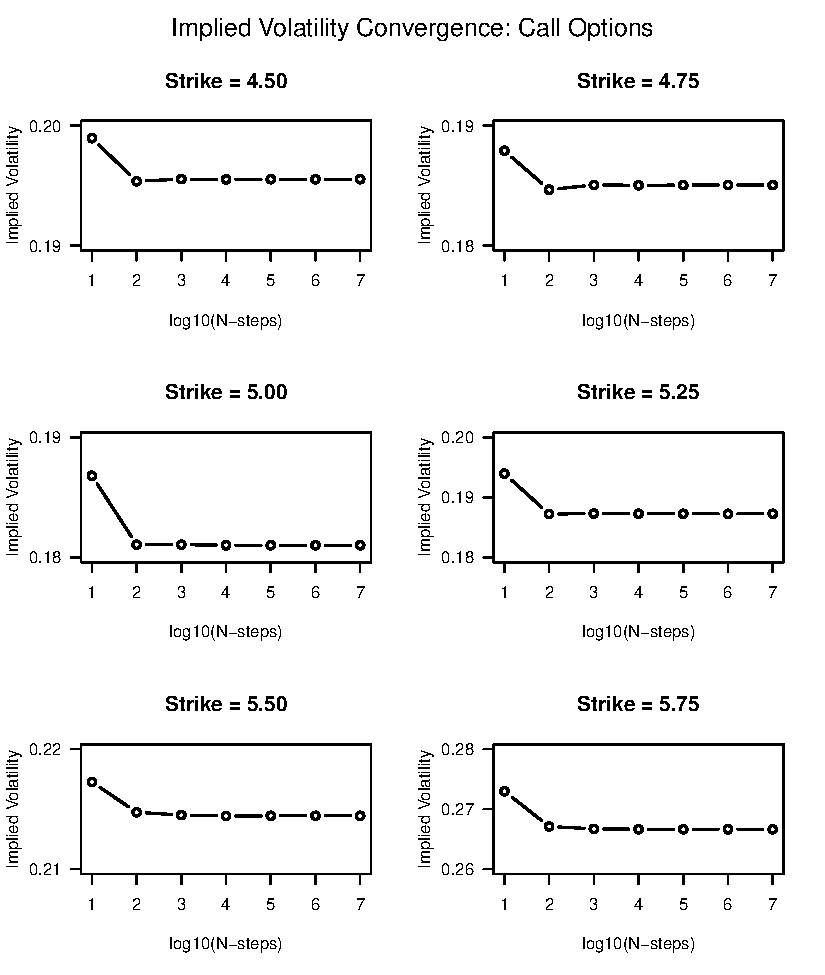
\includegraphics{../plots/call_convergence.pdf}
\caption{Implied volatility estimates given call option strike prices as a function of the $N$-steps of the binomial model. Qualitatively, convergence appears to occur relatively rapidly: By $N = 10^3$ little gains to volatility precision occurs.}
\label{fig:callconv}
\end{figure}
\begin{figure}[H]
	\centering
 	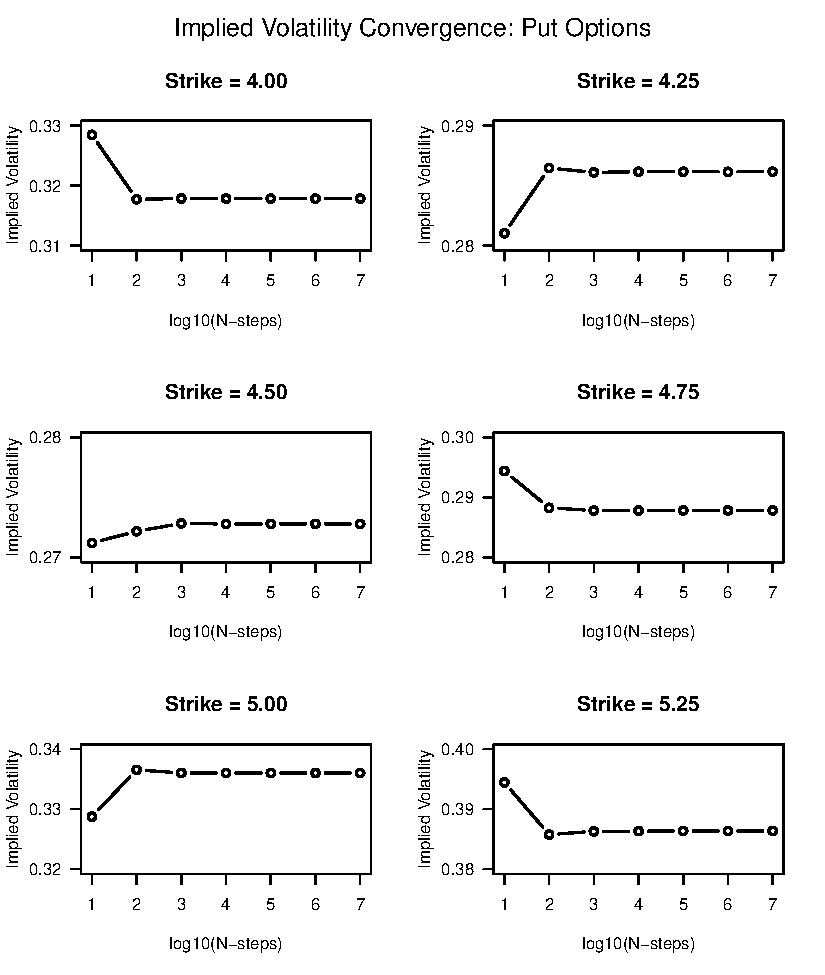
\includegraphics{../plots/put_convergence.pdf}
\caption{Implied volatility estimates given put option strike prices as a function of the $N$-steps of the binomial model. Similar to the volatility estimates of call options, convergence for puts appears by approximately $N = 10^3$.}
\label{fig:putconv}
\end{figure}
\begin{figure}[H]
	\centering
 	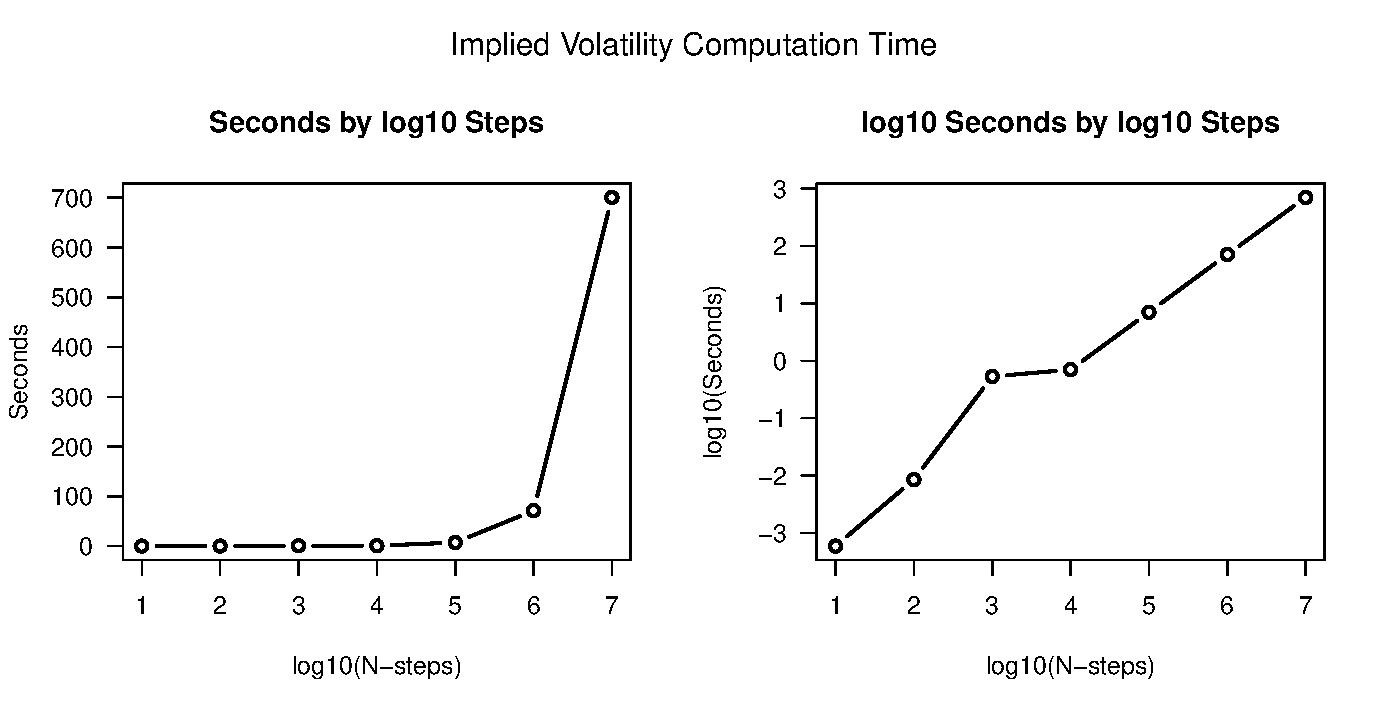
\includegraphics[scale=0.70]{../plots/times.pdf}
\caption{Run time as a function of the number of steps of the $N$-step binomial model. Given this particular algorithm we see nonlinear growth in time for $N \leq 10^3$ and linear growth in time for $N \geq 10^4$ when computing estimates of implied volatility.}
\label{fig:comptime}
\end{figure}

Figure \ref{fig:smile} gives us a visualization of the volatility estimates as a function of strike price. From this we immediately see the limitations of the binomial \& Black-Scholes models. These models assume that volatility is constant across strike prices and that volatility is independent of call and put contracts for a constant strike. However we see that neither of these assumptions hold for our computed implied volatilities. Not only is there the clear volatility smile, but we also see that put volatility estimates are across-the-board higher than the corresponding call estimates. A smile can be seen when considering only call or put contracts, but if constructing the smile from only out-of-the-money calls/puts then we see a discontinuity in the smile when the strike is contract is at-the-money.

\begin{figure}[H]
	\centering
 	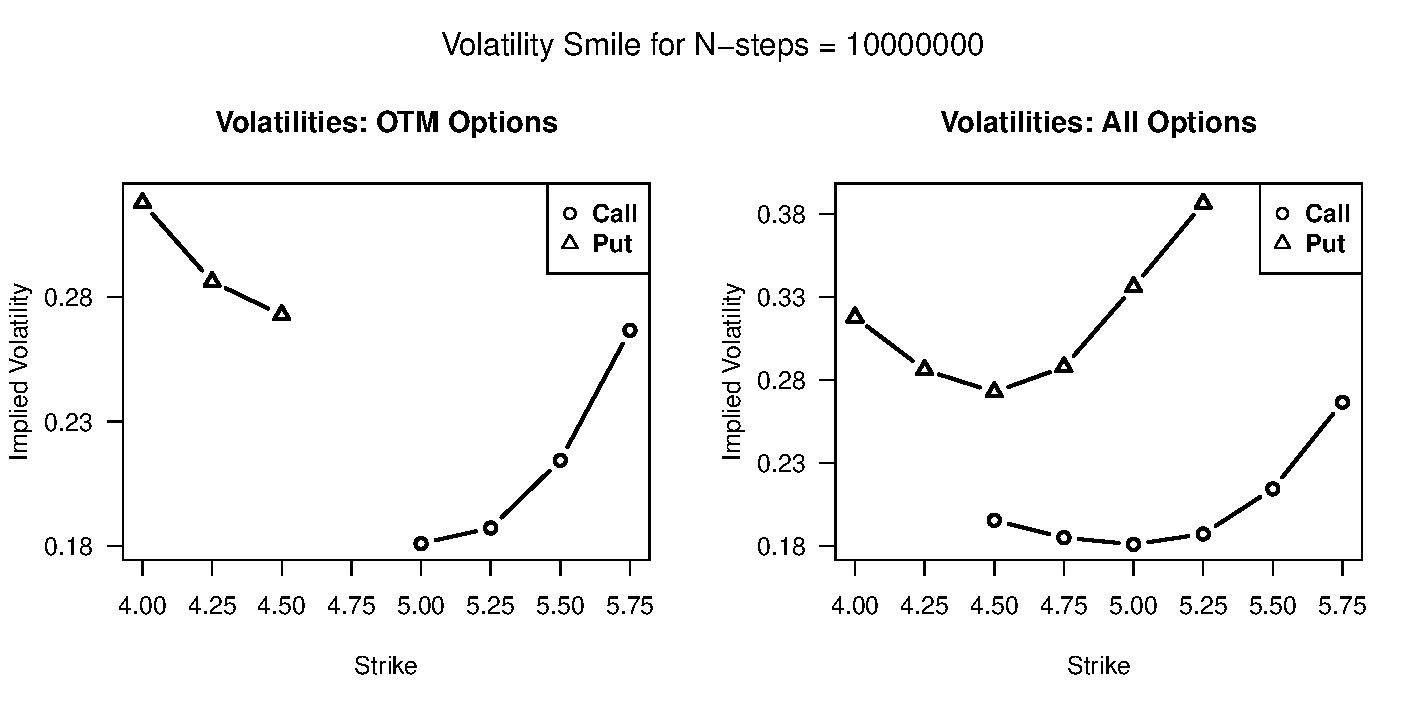
\includegraphics[scale=0.70]{../plots/smile.pdf}
\caption{Volatility estimates from the bisection algorithm of the binomial model plotted as a function of strike price. Left: Volatilities for out-of-the-money options. Right: Volatilities for all options. At the strike price corresponding to at-the-money options (\$4.75) note the discontinuity in implied volatility when considering only the out-of-the-money calls \& puts.}
\label{fig:smile}
\end{figure}


\newpage
\appendix
\section{Code Output: Data Table}\label{sec:data}

{\small
\csvautolongtable{../data/implied_vols.csv}
}
 
\newpage
\section{Code}\label{sec:code}
\subsection{Main.cpp}
\lstinputlisting{../code/Main.cpp}

\subsection{Asset.h}
\lstinputlisting{../code/Asset.h}
\subsection{Asset.cpp}
\lstinputlisting{../code/Asset.cpp}

\subsection{BinomialModel.h}
\lstinputlisting{../code/BinomialModel.h}
\subsection{BinomialModel.cpp}
\lstinputlisting{../code/BinomialModel.cpp}

\subsection{Option.h}
\lstinputlisting{../code/Option.h}
\subsection{Option.cpp}
\lstinputlisting{../code/Option.cpp}

\subsection{CallOption.h}
\lstinputlisting{../code/CallOption.h}
\subsection{CallOption.cpp}
\lstinputlisting{../code/CallOption.cpp}

\subsection{PutOption.h}
\lstinputlisting{../code/PutOption.h}
\subsection{PutOption.cpp}
\lstinputlisting{../code/PutOption.cpp}

\subsection{MathHelp.h}
\lstinputlisting{../code/MathHelp.h}
\subsection{MathHelp.cpp}
\lstinputlisting{../code/MathHelp.cpp}


\subsection{makeplots.R}
\lstinputlisting[language=R]{../code/makeplots.R}


\end{document}
























